\documentclass[%
aip,
jmp,
reprint,
floatfix,
]{revtex4-1}

\usepackage{graphicx}% Include figure files
\usepackage{float}
\usepackage{siunitx}
\usepackage{hyperref}
\usepackage{listings}
\usepackage[english]{babel}
\usepackage[utf8]{inputenc}
\usepackage{ gensymb }
\usepackage{color}
\usepackage{subcaption}
\usepackage{csvsimple}

\definecolor{dkgreen}{rgb}{0,0.6,0}
\definecolor{gray}{rgb}{0.5,0.5,0.5}
\definecolor{mauve}{rgb}{0.58,0,0.82}

\lstset{
	frame=single, 
	language=Python, 
	columns=flexible,
	basicstyle={\footnotesize\ttfamily},
	keywordstyle=\color{blue},
	commentstyle=\color{dkgreen},
	stringstyle=\color{red},
	title=\lstname
}


\renewcommand{\arraystretch}{1.3} % Changes the height of tables
\DeclareSIUnit\year{yr}
\DeclareSIUnit\parsec{pc}
\DeclareSIUnit\day{d}



\begin{document}

	\title[Solar Rotation]{Solar Rotation}

	\author{Lucas, Miles}
	\affiliation{Iowa State University Department of Physics and Astronomy}

	\date{\today}


% Write here a short abstract (1 paragraph) describing what you achieved in this lab.

	\begin{abstract}
	This report seeks to characterize the rotational period of the Sun. We used \SI{6173}{\angstrom} SDO data and measured the pixel location of sunspots over a range of time from \date{2014 October 20} to \date{2014 October 29}. This data is fit using a linear regression. From the fit I calculated the synodic period to be \SI{26.181 \pm .059}{\day} and the sidereal period to be \SI{24.430 \pm .051}{\day}.
	\end{abstract}

	\maketitle
%________________________________________________________________________

%	Write here a summary of the goals of this lab. Be brief – do not exceed the end of the first page.

	\section{Introduction}
	The goal of this lab is to determine the sidereal solar rotation rate and period. To accomplish this, I used solar images from October of 2014 and will trace a sunspot's motion from day to day. 
	
	In order to determine the motion of the sunspots, I used a simple cosine function to describe its motion.
	\begin{equation}
	x = R \cos{\omega t + \delta}
	\label{eqn:wave}
	\end{equation}
	where $x$ is the distance of the spot from the meridian and $R$ is the distance from the meridian to the limb. \autoref{fig:pos} shows this relationship.
	
	In order to evaluate the frequency of rotation, $\omega$, I linearized \autoref{eqn:wave} with respect to $t$
	\begin{equation}
	\omega t + \delta = \arccos{x/R}
	\label{eqn:line}
	\end{equation}
	
	This function can be easily fit with a linear regression and the reported synodic frequency, in \si{\per \day}, can be given as 
	\begin{equation}
	\omega = \hat{\omega} \pm \hat{\omega} \cdot S
	\label{eqn:err}
	\end{equation}
	where $\hat{\omega}$ is the estimator for the slope and $S$ is the standard error of the fit.
	
	Also, to account for the motion of the Earth around the sun, we use the simple relation
	\begin{equation}
	\frac{1}{T_{sid}} = 1 + \frac{1}{T_{syn}}
	\end{equation}
	
	\begin{figure}
		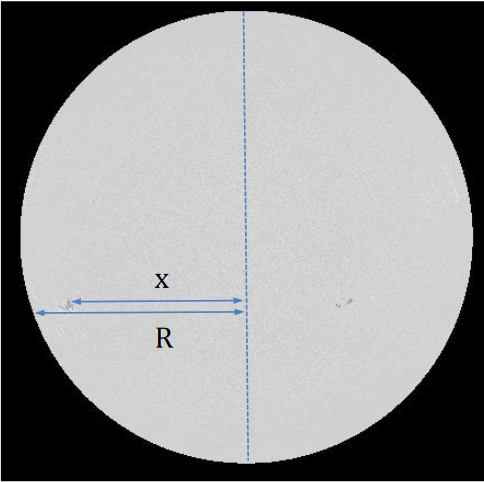
\includegraphics[width=.9\linewidth]{figs/pos.png}
		\caption{A visual of the limb width and sunspot location from each solar image}
		\label{fig:pos}
	\end{figure}
%________________________________________________________________________

%	Describe your telescope and camera setup. For the first lab you should describe the setup in more details. Subsequent labs can refer to the procedure described in the first lab, and focus more on the data acquisition itself. Important details to write include: which stars have been observed, which filters were used (BVI), what exposure times and what calibration procedures have been followed (e.g., dark frames acquisition, photometric standards observed, etc.). Mention also the observing conditions (weather, moon presence, temperature, etc.). You should include the observing log appendix A (a table or a scan of a hardcopy). This section can be as long as necessary, but you should strive for brevity (you can refer to the lab guide to avoid repeating all steps, but make sure you explain anything you did differently, problems encountered, etc.). Use tables to summarize information clearly.

	\section{Data Acquisition}
	The images were all obtained from with courtesy from SolarMonitor.org. The images obtained were \SI{6173}{\angstrom} images caputred using the Solar Dynamics Observatory's (SDO) Helioseismic and Magnetic Imager (HMI). The HMI allows stabilized \SI{1}{\arcsecond} full-disk images of the sun. 
	
	SolarMonitor.org accumulates different solar image sources every day and displays them neatly on their website. From here it is easy to select a solar source, pick a date for observation, and download the FITS data file for the image. 
	
	I chose images from 2014 due to the heightened solar activity and found a large sunspot around October 31. I found 10 neighboring images that contained the sunspot and ended with a range of images from 2014 October 19 to 2014 October 29. \autoref{fig:sun} shows examples of images from two dates within this range.
	
	\begin{figure*}[t]
		\centering
		\begin{subfigure}[]{.4\textwidth}
			\centering
			\includegraphics[width=\textwidth]{figs/20141021.png}
			\caption{\SI{6173}{\angstrom} image from \date{2014 October 21}}
		\end{subfigure}
		\qquad
		\begin{subfigure}[]{.4\textwidth}
			\centering
			\includegraphics[width=\textwidth]{figs/20141027.png}
			\caption{\SI{6173}{\angstrom} image from \date{2014 October 27}}
		\end{subfigure}
		\caption{Example pictures showing sunspot traced sunspot}
		\label{fig:sun}
	\end{figure*}
%________________________________________________________________________

%Describe what you did to analyze the data. For the first lab this section will be minimal. For subsequent labs you should describe in detail the steps you did to analyze the data.  If applicable you can attach the code you used to analyze the data in Appendix B (either a log of your IDL section, or the code of any scripts you wrote). You can also attach screenshots of your computer session if it helps your discussion. Include tables of raw data in this section. The goal of this section is to describe unambiguously what you did to derive your final images and measured quantities from the raw data. Again be brief but complete (use as much space as you need).
	\section{Data Analysis}
	To find the sunspot positions I loaded the 10 images into SAO's ds9. I started by finding what the meridian pixel value was, because the image is laid out from (0, 0) in the top-left and extending down and to the right. 
	
	I picked what I thought the center of the sunspot of interest was and noted the y-position. This should stay consistent from each image. I then measured the meridian to limb length ($R$) with the first image and then found the relative position of the sunspot in each image to the meridian. 
	
	I also used \autoref{lst:dateparse} to parse the dates from the headers of the FITS files and construct the data table. Into this table I recorded all of the relevant position values. 
	
	Then, using this table, I used python to do a linear regression of \autoref{eqn:line}. The python library uses a simple least-squares fit. 
	
%________________________________________________________________________

%	Describe in detail the results you obtained from the quantitative analysis of your data, as explained in the lab guide.
	\section{Results and Discussion}
	
	The measurements from each image are listed in \autoref{tab:data}. The linear fit is shown in \autoref{fig:line}. The uncertainties were found using least squares propagation methods where the absolute uncertainty for the synodic frequency is shown in \autoref{eqn:err}. From this fit, I report the synodic period to be \SI{26.181 \pm .059}{\day} and the sidereal period to be \SI{24.430 \pm .051}{\day}. This is of the same magnitude as the accepted values for solar rotation, where my errors arise from approximation in sunspot position, especially with the distortion as it approaches the limb.

	\begin{table}
		\centering
		\caption{Sunspot Position Information}
		\csvreader[
		tabular=lllrr, 
		table head=\hline Date & Time & MJD & x & x/R \\ \hline\hline, 
		table foot=\hline]
		{../data/table.csv}{}{\csvcolii & \csvcoliii & \csvcoliv & \csvcolvi & \csvcolvii}
		\label{tab:data}
	\end{table}

	\begin{figure*}[t]
		\centering
		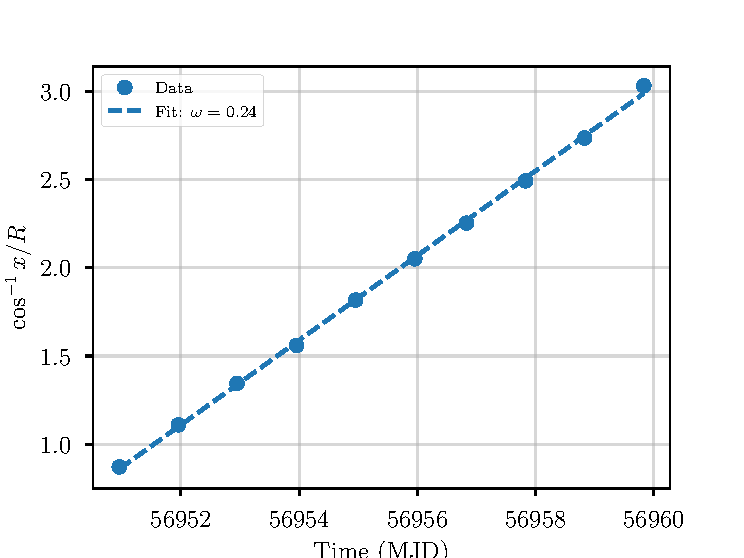
\includegraphics[width=.8\linewidth]{figs/fit.pdf}
		\caption{Linear fit of the linearized data showing the synodic frequency of the sun in \si{\per\day}.}
		\label{fig:line}
	\end{figure*}

%________________________________________________________________________

%	Add here anything else you want to say, and summarize your results. This section should be very brief, not more than a couple of paragraphs
%	\section{Conclusions}
	


%________________________________________________________________________

	\section*{Acknowledgments}

	Thank you to Dr. Charles Kerton and Brandon Marshall for their guidance and assistance in this work. Also, thank you to SolarMonitor.org and Solar Dynamics Observatory for their open source data.


%________________________________________________________________________

	\onecolumngrid
	\appendix

	\section{Analysis Scripts} \label{sec:scripts}
	Also see Jupyter Notebook at \href{https://github.com/mileslucas/astro344l/blob/master/lab7/src/lab7.ipynb}{this Github page}.
	\lstinputlisting[label={lst:dateparse}]{../src/parse_dates.py}
	
	

\end{document}
